\documentclass[12pt, letterpaper]{article}
\usepackage[utf8]{inputenc}
\usepackage{graphicx}
\usepackage{amsmath}
\title{Conditional Stochastic Layers}
\date{}

\begin{document}
\vspace{-5cm}
\maketitle
\vspace{-2cm}


\section{Physical Incarnations}
We categorize the conditional stochastic layers based on their architecture.
Any trainable network or layer(s) with trainable parameters can act as conditional stochastic layers. 
These include (but are not limited to) convolutional layers, fully connected layers, support vector machines, recurrent networks like LSTMs, transformers, etc. In this section we discuss convolutional conditional stochastic layers and fully connected conditional  stochastic layers as physical incarnations of the conditional stochastic layers. 
\subsection{Convolutional Conditional Stochastic Layers}

\textbf{Convolutional Layers}: Convolution (in the context of neural networks) is a linear mathematical operation where a kernel $k$ slides across an input tensor $x$ performing a linear operation at every location of the tensor, thereby transforming the tensor in a certain way. 
The output of this operation is a tensor $h_k$ which represents a feature (also called an activation). 
In a convolutional layer of a neural network, the input tensor $x$ is passed through a number of kernels, whose parameters are learnt during training through backpropagation. 
The activations $h_k$ from the respective kernels $k$ are stacked into channels to form the output $h=[h_k]$. Eq.~\eqref{eq:conv} shows the convolution operation. 
In Eq.~\eqref{eq:conv}, $[m,n]$ represents the spatial coordinates of the output tensor $h_k$, $[i,j]$ represents the spatial coordinates of the kernel $k$.
\begin{equation}
  h_k[m,n]=(x * k)[m,n]=\sum_i \sum_j k[i,j]x[m+i,n+j]
  \label{eq:conv}
\end{equation}

\noindent \textbf{Convolutional Conditional Layers}: Deep networks are often employed for tasks that involve categorizing objects into a specific category from the training dataset. For example, object classification involves determining whether a given image is of a cat or a dog. Object detection involves the same, with the additional task of localizing the animal spatially. It is often useful to learn convolutional kernels specific to the category of objects. In other words, convolutional layers can be conditioned on the category of object. This is shown in Eq.~\eqref{eq:condconv}, where $k_c$ represents the kernels specific to the category $c$ in the training dataset.

\begin{equation}
  h_{k_c}[m,n]=(x * k_c)[m,n]=\sum_i \sum_j k_c[i,j]x[m+i,n+j]
  \label{eq:condconv}
\end{equation}
\begin{figure}[t]
    \centering
    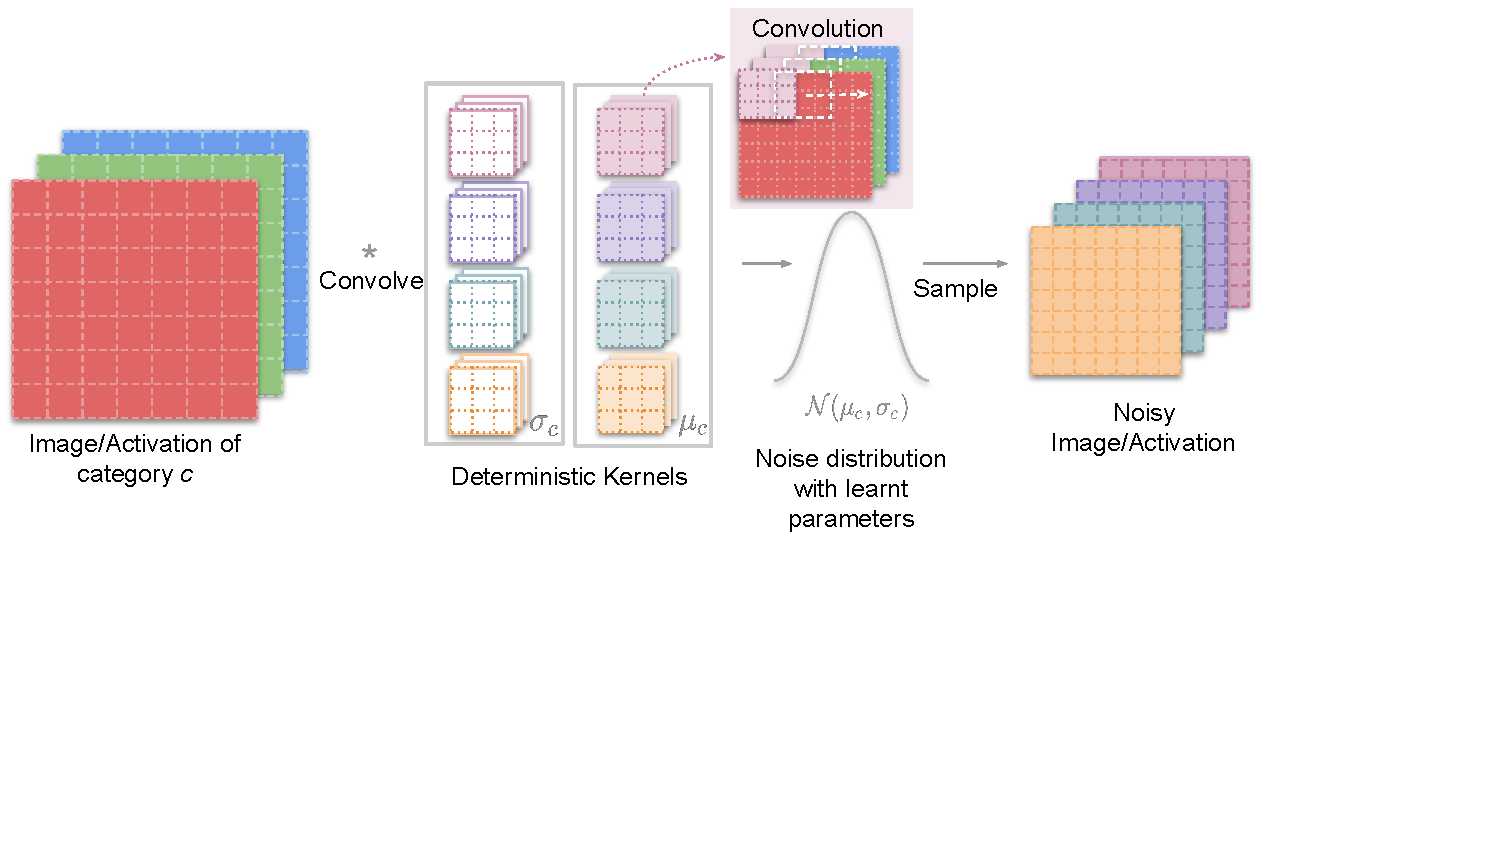
\includegraphics[width=\textwidth, trim={0 5cm 2.5cm 0}, clip]{Conditional noise layer.pdf}
    \caption{Conditional convolutional stochastic layer with learnt kernels $\mu_c$ and $\sigma_c$. The conditional probability distributions $\mathcal{N}(\mu_c, \sigma_c)$ are conditioned on the image category or label $c$.}
    \label{fig:condconv}
\end{figure}

\noindent \textbf{Convolutional Conditional Stochastic Layers}:
To introduce stochasticity, the output activations ($h_{k_c}$ in Eq.~\eqref{eq:condconv}), obtained as a result of the convolution operation between input $x$ and kernels $k_c$, acts as parameters of a probability distribution. 
Any probability distribution is applicable according to the use case including (but not limited to) gaussian, binomial and multinomial distributions.  
Fig.~\ref{fig:condconv} shows the mechanism where the kernels convolve over an input to produce the parameters of a gaussian distribution. Instead of following the usual practice of using $h_{k_c}$ in Eq.~\eqref{eq:condconv} directly as inputs to the next layers, we sample from the parameterized probabibility distribution and use this sample as an input to the next layer. This is elaborated in Sec.~\ref{sec:training_inf}.

\subsection{Fully Connected Conditional Stochastic Layers}
\textbf{Fully Connected Layers:} A fully connected layer performs the inner-product between the input activation vector ($x$) and the trainable parameter vector $W$.
This is represented by Eq.~\eqref{eq:linear}. The vector $h$ represents the output activation that propagates forward.
\begin{equation}
h=W \cdot x
    \label{eq:linear}
\end{equation}

\noindent \textbf{Fully Connected Conditional Layers}: It is often useful to learn weights $W_c$ specific to the category of objects given in the training dataset. In other words, fully connected layers can be conditioned on the category of object. This is shown in Eq.~\eqref{eq:condlinear}, where $W_c$ represents the weights specific to the category $c$ in the training dataset.

\begin{equation}
h_c=W_c \cdot x
    \label{eq:condlinear}
\end{equation}

\noindent \textbf{Fully Connected Conditional Stochastic Layers}:
To introduce stochasticity, the output activations ($h_c$ in Eq.~\eqref{eq:condlinear}) obtained as a result of the inner product between the input $x$ and weights $W_c$ acts as parameters of a probability distribution. 
Any probability distribution is applicable according to the use case including (but not limited to) gaussian, binomial and multinomial distributions.  
Instead of using $W_{c}$ in Eq.~\eqref{eq:condlinear} directly as inputs to the next layers, we sample from the probabibility distribution and use the sample as an input to the next layer. This is elaborated in Sec.~\ref{sec:training_inf}.

\section{Training and Inference}
\label{sec:training_inf}
 
In this section, we elaborate the training and inference procedures for the conditional stochastic layers, considering the convolutional incarnation and by assuming a gaussian distribution for the output activations for the task of multi-class classification. Other physical incarnations, types of distributions and applications will have identical procedures. We describe several applications in Sec.~\ref{sec:app}


\subsection{Training} 
We describe training as a $2$ step procedure. In the first step, we learn the weights of the conditional stochastic layer. In the next step, we learn category masks that are necessary during inference. The steps are described below. Note that the training pipeline can be different depending on application. For example, step 2 can be omitted if the user is aware of the class labels when the image/activation is passed through the conditional stochastic layer. Fig.~\ref{fig:classification} describes a forward pass during the training procedure.

\noindent \textbf{Training of Conditional Stochastic Layer:}
Prior to training, two sets of kernels ($k_{\mu_c}$ and $k_{\sigma_c}$) are initialized for the two parameters in a gaussian distrubution $\mu_c$ and $\sigma_c$ respectively, conditioned on each category $c$ in the training dataset. During the forward pass, the kernels $k_{\mu_c}$ and $k_{\sigma_c}$ perform convolution operation on the input activation $x$, if $x$ belongs to the category $c$. In other words, $x$ is first multiplied with a category mask $\pi_c$, which is $1$ if $x$ belongs to category $c$, and $0$ if $x$ belongs to any other category. This modified input is then passed through the conditional stochastic layer. The output activation maps ($\mu_c$ and $\sigma_c$) are obtained from the respective set of kernels according to Eq.~\eqref{eq:mu_c} and Eq.~\eqref{eq:sigma_c}. $\mu_c$ and $\sigma_c$ are used to define the gaussian distribution. We randomly sample an activation map  $h_c$ from this distribution according to Eq.~\eqref{eq:sample}. $h_c$ acts as an input activation for the next layers in the network. 

\begin{equation}
  \mu_c[m,n]=(x * k_{\mu_c})[m,n]=\sum_i \sum_j k_{\mu_c}[i,j]x[m+i,n+j]
  \label{eq:mu_c}
\end{equation}
\begin{equation}
  \sigma_c[m,n]=(x * k_{\sigma_c})[m,n]=\sum_i \sum_j k_{\sigma_c}[i,j]x[m+i,n+j]
  \label{eq:sigma_c}
\end{equation}

\begin{align}
  h_\mathrm{c} \sim \mathcal{N}(\mu_c,\sigma_c) \notag\\
  \Rightarrow h_c=\mu_c + \sigma_c.\epsilon;\; \epsilon \sim \mathcal{N}(0,1)
  \label{eq:sample}
\end{align}

The kernels are trained in a similar manner as standard convolutional neural networks. The parameters of the gaussian distribution for each category $\mu_c$ and $\sigma_c$ (Eq.~\eqref{eq:mu_c} and Eq.~\eqref{eq:sigma_c}), obtained in the forward pass, are differentiable with respect to the kernels $k_{\mu_c}$ and $k_{\sigma_c}$ respectively. $h_c$ is differentiable with respect to $\mu_c$ and $\sigma_c$. Gradients of the output activation $h_c$ can be obtained with respect to the kernels  $k_{\mu_c}$ and $k_{\sigma_c}$. The kernels are trainable using the aforementioned gradients through back-propagation and gradient descent. 

\noindent \textbf{Training of Category Masks:}
The category masks can directly be applied to the input $x$. As other embodiments, the category masks can also be applied after the stochastic layers, or anywhere in the neural network. We describe the training procedure considering that the category masks are applied directly on the input.

The input $x$ is multiplied with trainable category masks $\pi_c$ whose values vary between $0$ and $1$, representing the probability of the image belonging to a certain category $c$. If there are $C$ categories in the dataset, there are $C$ category masks to be trained. $\pi=\{\pi_c\}$ represents all the category masks concatenated together. The modified input ($x \odot \pi$) undergoes forward pass. The activations at every step are differentiable with respect to the category masks and hence backpropagation and gradient descent are directly applicable to train the category masks.
The step involving training of the category masks can be omitted if the user is aware of the input category when the input is passed through the conditional stochastic layer. In that case, we use $\pi_c=1$ if $x$ belongs to category $c$, otherwise $\pi_c=0$. 


\subsection{Inference}
The kernels $k_{\mu_c}$ and $k_{\mu_c}$ and category masks $\pi_c$ are trained according to the previous sub-section. A forward pass is performed using the category masks and trained kernels to produce the a parameterized probability distribution, from which the output activation map $h_c$ is sampled. The output activation map acts as an input activation for the next layer in the neural network. 
\section{Applications}
\label{sec:app}
Conditional stochastic layers are useful for multi-class classification, multi-object detection, semantic and instance segmentation, multi-object tracking, and many more applications. We elaborate multi-object detection and multi-class classification applications in this section. We also demonstrate how conditional stochastic layers can be used in the context of federated learning for multi-class image classification. Note that, this process is applicable to other use-cases.

\subsection{Multi-Class Object Classification}

\begin{figure}[h!]
    \centering
    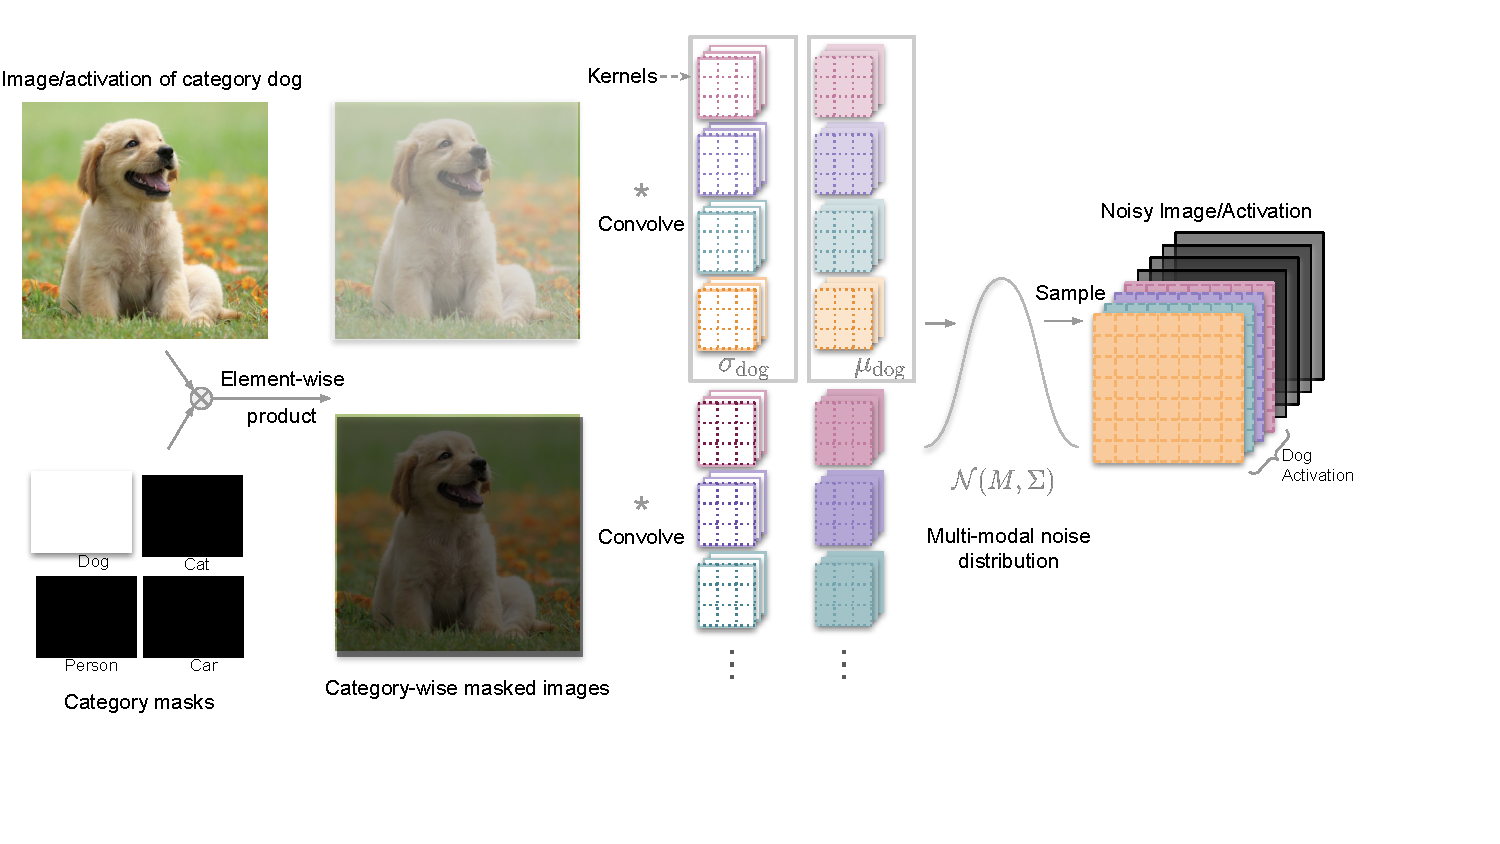
\includegraphics[width=\textwidth, trim={0cm 2cm 2.4cm 0.5cm}, clip]{Classification Conditional noise layer.pdf}
    \caption{Conditional convolutional stochastic layer for multi-class classification. The multi-modal conditional probability distribution $\mathcal{N}(M, \Sigma)$, where $M=\{\mu_c\}$ and $\Sigma=\{\sigma_c\}$) is used to sample the output activation. $\mu_c$ and $\sigma_c$ are conditioned on the image category or label $c$ ($c=$dog in this case). During training, the category mask $\pi_\{mathrm{dog}$ is $1$. All other category masks are $0$. Trained category masks are used during inference.}
    \label{fig:classification}
\end{figure}
Multi-Class Object Classification is the task of categorizing an image into one class or category, when the training dataset contains multiple categories. The training and inference procedure is described in Sec.~\ref{sec:training_inf}.

There are $C$ category masks if there are $C$ total categories in the training datasets. Each category mask is element-wise multiplied with the input $x$ before being convolved with all the convolutional kernels. 
The pixel of the category masks used during training of kernels have the value of 1 if the image matches the certain category. Otherwise, the pixel value is 0. This ensures that the given image of category $c_1$, only passes through kernels $\mu_c$ and $\sigma_c$, and no other sets of kernels, when the input image $x$ is element-wise multiplied with each category mask.

After the kernels are fully trained, optimal category masks are trained (Sec.~\ref{sec:training_inf}). Each pixel represents a probability that the particular region is of interest, and hence has a value between $0$ and $1$. The trained category masks are used for inference. 

\subsection{Multi-Object Detection}
\begin{figure}[h!]
    \centering
    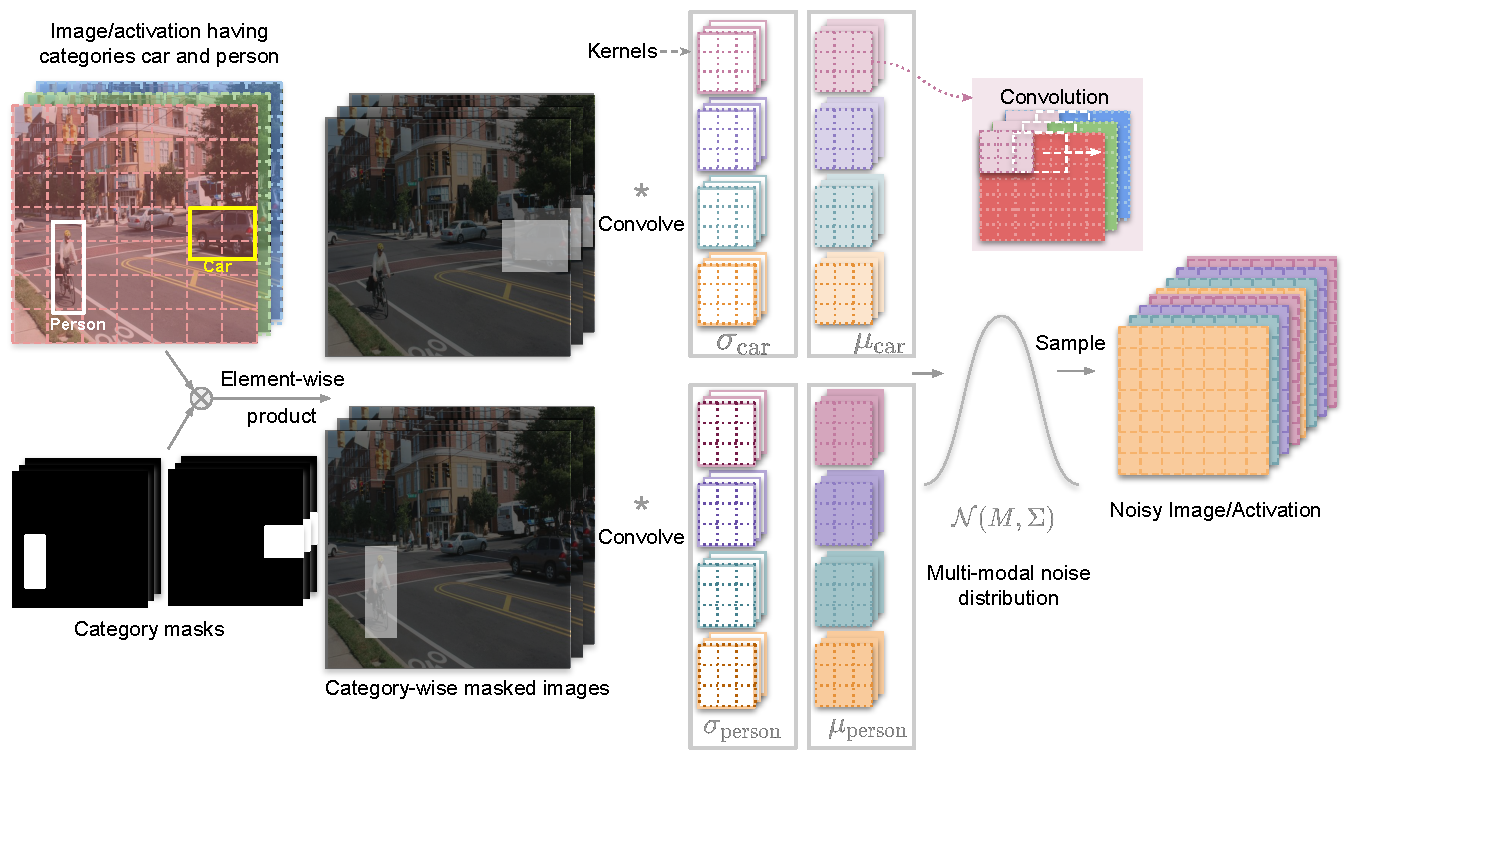
\includegraphics[width=\textwidth, trim={0cm 1.6cm 2.7cm 0cm}, clip]{Detection Conditional noise layer.pdf}
    \caption{Conditional convolutional stochastic layer for multi-object detection. The multi-modal conditional probability distribution $\mathcal{N}(M, \Sigma)$, where $M=\{\mu_c\}$ and $\Sigma=\{\sigma_c\}$) is used to sample the output activation. $\mu_c$ and $\sigma_c$ are conditioned on the image category or label $c$ ($c$ is person or car in this case). The category masks $\pi_c$ have pixel values $0$ or $1$ during training, depending on the region of interest of category $c$. Trained category masks are used during inference.}
    \label{fig:det}
\end{figure}

\begin{figure}[h!]
    \centering
    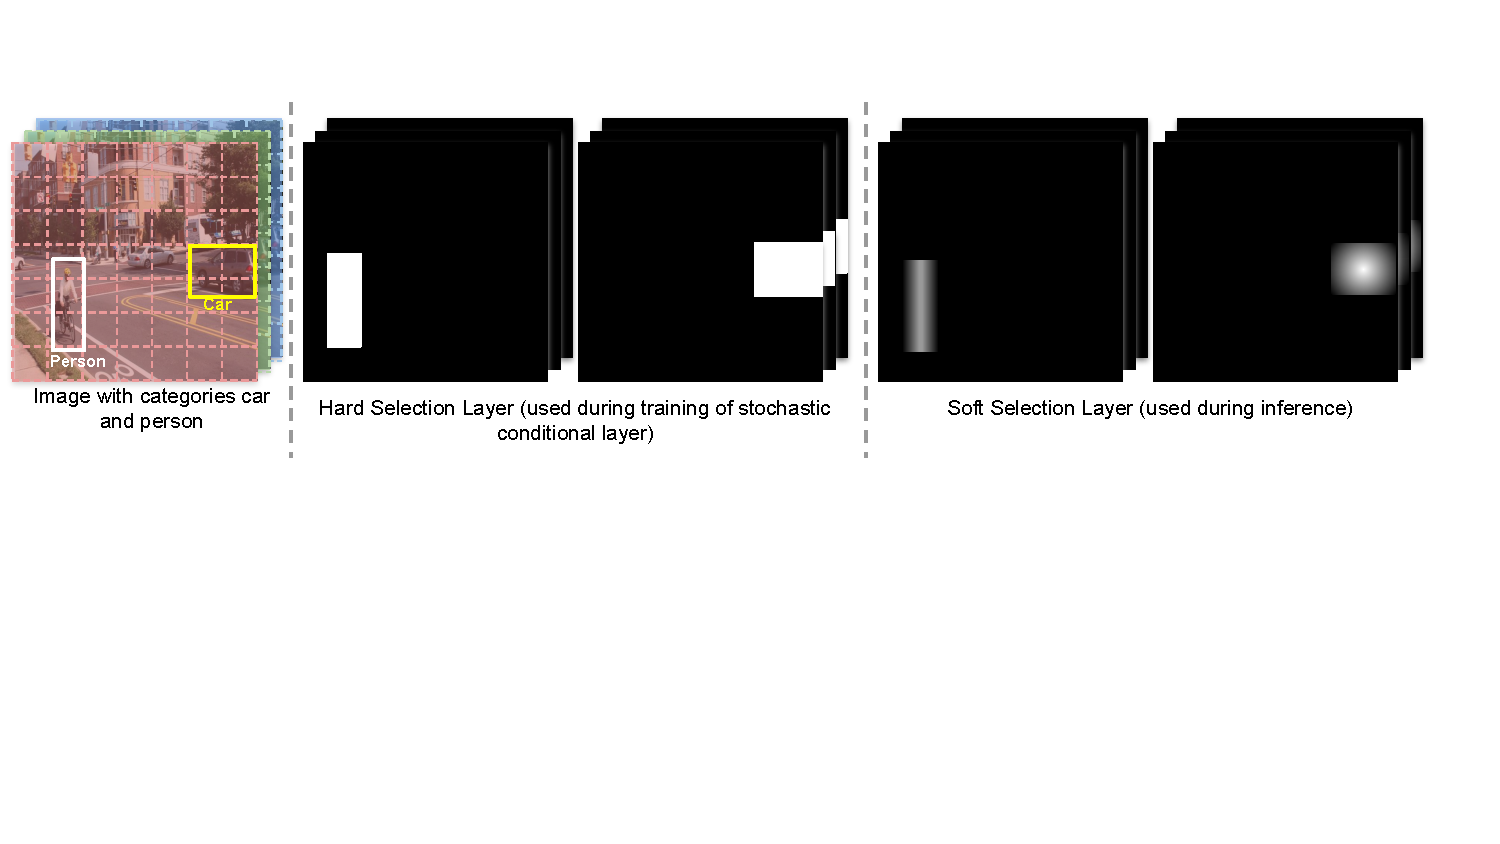
\includegraphics[width=\textwidth, trim={0cm 7cm 1cm 2cm}, clip]{category_masks.pdf}
    \caption{Category masks used during training and inference. During training, pixel values are either $0$ or $1$. Trained category masks are used during inference, where pixel values vary between $0$ and $1$, representing the  probability that the particular pixel in category mask $\pi_c$ belongs to class $c$.}
    \label{fig:category_masks_det}
\end{figure}

Multi-Object detection is the task of categorizing and localizing multiple objects, given an image. For example, objects of the categories ``person'' and ``car'' are to be detected in the input image shown in Fig.~\ref{fig:det}. The training and inference procedure is described in Sec.~\ref{sec:training_inf}.

The category masks used during training of kernels is shown in Fig.~\ref{fig:category_masks_det} (middle figure). The white pixels indicate the value of 1, and black pixels indicate the value of 0. This ensures that the regions of interests are retained when the input image $x$ is element-wise multiplied with each category mask.

After the kernels are fully trained, optimal category masks are trained (Sec.~\ref{sec:training_inf}). Each pixel represents a probability that the particular region is of interest for a certain category. The trained category masks, (Fig.~\ref{fig:category_masks_det} (right)) are used for inference. 

\subsection{Federated Learning}

We discuss learning of the stochastic noise layer in the federated learning setting. Any task like multi-class classification, multi-object detection, etc, can be considered for this. We discuss one embodiment of the federated learning procedure on the task of multi-class classification. Other embodiments follow similar procedure.

\begin{enumerate}
    \item We train a given neural network on 5\% of the training dataset, instead of the entire dataset. Let us call this trained neural network NN-5.
    \item We use NN-5 to train the conditional stochastic layer described earlier. We call this stochastic layer SL-5.
    \item We already have 5\% of the pure dataset. We obfuscate the rest 95\% of the training data using SL-5 and regulariztion technique described in Sec.~\ref{sec:reg}.  
    \item We then resume training of NN-5 on this 5\% pure and 95\% noisy dataset (obtained from the previous step). Let's call this trained neural network NN’-5.
    \item We gradually make more training data available (10\%, 15\%, etc) and iterate over steps 1,2,and 3, until the desired accuracy is reached.
\end{enumerate}

\subsubsection{Regularization}
\label{sec:reg}
In step 3 of the federated learning embodiment described above, we obfuscate 95\% of the training data using a stochastic layer training on only 5\% of the pure training dataset (SL-5). Note that this noisy data coming from the stochastic layer will be highly biased towards the small ratio of the data SL-5 was trained on. To reduce this bias, we propose a regularization step where we randomly screen parts of the noisy data at every iteration of the training, so that the screened parts aren't visible to the neural network. 


\section{Related Work}
Previous works attempted to ensure that the accuracy of the deep networks trained on very little carefully crafted or chosen training data, remain similar to the accuracy of the deep networks trained on full training datasets. Some of these attempts are described next.

\noindent \textbf{Dataset distillation:} Wang et al.~\cite{datasetdistillation} learned a small number of data points that do not need to come from the correct data distribution.  A model trained on these synthetic data points approximate a model trained on the original data well.

\noindent \textbf{Active learning:} Active learning \cite{al1,al2,al3,al4} attempts to maximize the performance of models while annotating very little training data. The deep model is first trained using a small set of annotated training data.  The model queries a user to label selected unlabelled samples for which the model had the lowest prediction confidence. 


{\small
\bibliographystyle{ieee_fullname}
\bibliography{egbib}
}

\end{document}
